
\chapter{Results}\label{results}

\section{Behavioral results}

If not noted otherwise, two comma-separated values in brackets describe the upper and lower values of a 95\% confidence interval.

\subsection{Response times}

A Shapiro-Wilk test was conducted to determine if individual response times were normal distributed.
All subjects failed this test (p < 0.001), indicating a strong deviation from normality.
Therefore, I represented individual response times by their median.

Children needed a median time of 1.91s (1.64s, 2.19s) to respond to object-relative clauses.
For subject-relative clauses, they needed 1.97s (1.69s, 2.25s).
Adults needed a median time of 1.51s (1.28s, 1.73s) to respond to object-relative clauses.
For subject-relative clauses, they needed 1.60s (1.37s, 1.82s).

A Shapiro-Wilk test determined that response time data was normal distributed with a probability between 1.5\% and 27\%.
A Levene's test determined that the probability of median response times being normal distributed was ?\%.
Supported by these findings, the response times were included into the ANOVA.

\subsection{Response accuracy}

For the analysis of variance (ANOVA), all data must be normal distributed with equal variance.
A Shapiro-Wilk test determined that the probability of accuracy data being normal distributed was between 2.0 and 20.3\%.
A Levene's test yielded that the probability that accuracy data were distributed with equal variance was less than p = 0.1\%.

The ANOVA is known to be robust for considerable deviations from the normal distribution.
However, it is highly vulnerable to violation the assumption of equal variances.
To meet this requirement, I transformed the accuracy data with the inverse sigmoid function.
This procedure, however, created singularities in some extreme cases, i.e., when a subject performed with a 100\% accuracy rate.
To prevent this issue, I added a single incorrect trial to every subject's performance for the following analysis.

After the transformation, the same tests as before were conducted.
The probability for transformed accuracy data being normal distributed was between 0.5\% and 27\%.
The probability for transformed accuracy data being distributed with equal variance was p = 72.2\%.
Supported by these findings, the transformed accuracy data was included in the ANOVA.

\subsection{Analysis of combined performance data}

Two ANOVA were conducted with the transformed accuracy data and the median response times.
Each subject provided one data point for each metric.
Data were analyzed with a group x condition design.
Accuracy estimates were transformed back with the sigmoid function $r = \frac{1}{1+e^{\hat{-r}}}$.

Children responded 0.39s slower than adults (1.94s vs. 1.55s).
This difference was significant ($F_{56} = 9.4$, $p = 0.3\%$).

Children responded with an average accuracy of 93.8\% (92.2\%, 95.0\%).
Adults performed much better, with an average accuracy of 97.9\% (97.5\%, 98.3\%).
This difference was highly significant ($F_{56} = 52$, $p = 1.6*10^{-9}$).

Sentence condition had no impact on median response times ($F = 0.33$, $p = 57\%$) or on response accuracy ($F = 1.3$, $p = 26\%$).
There was no interaction effect between group and sentence condition ($F < 0.1$, $p > 80\%$).

\section{Sensor-space activity}

We computed average event-related fields (ERF) for each subject and sensor region.
Activity from these ERF was selected with two different types of time windows.

A positive effect indicates that activity evoked by object-relative clauses was more positive than activity evoked by subject-relative clauses. In the case of gradiometers, "'more positive"' means a higher regional RMS. With localized data, "'more positive"' means a higher z-score from the sLORETA source reconstruction.


\subsection{Interval analysis}
For this analysis, sensor activity from separate regions and hemispheres was compared blindly between 0 and 2200ms after onset in 200ms intervals.

After FDR-correction for 10 comparisons, no sensor region showed any non-spurious effect in either group ($p > 3\%$).

\subsection{Cluster analysis}
For this analysis, activity was compared between conditions using a temporal cluster analysis.

For children, significant differences were observed in the following sensor groups:
Right parietal magnetometers showed a negative effect between 159ms and 374ms ($p = 1.4\%$).
Left frontal magnetometers showed a negative effect between 375ms and 666ms ($p = 1.8\%$).
Left temporal magnetometers showed a negative effect between 349ms and 627ms ($p = 0.8\%$).
Right temporal gradiometers showed a positive effect between 1384ms and 1663ms ($p = 3.8\%$).
This activity can be summarized into two time windows: a negative effect between 159ms and 666ms, and a positive effect between 1426ms and 1663ms.

\begin{figure}[h]
\begin{center}
\vspace{7mm}
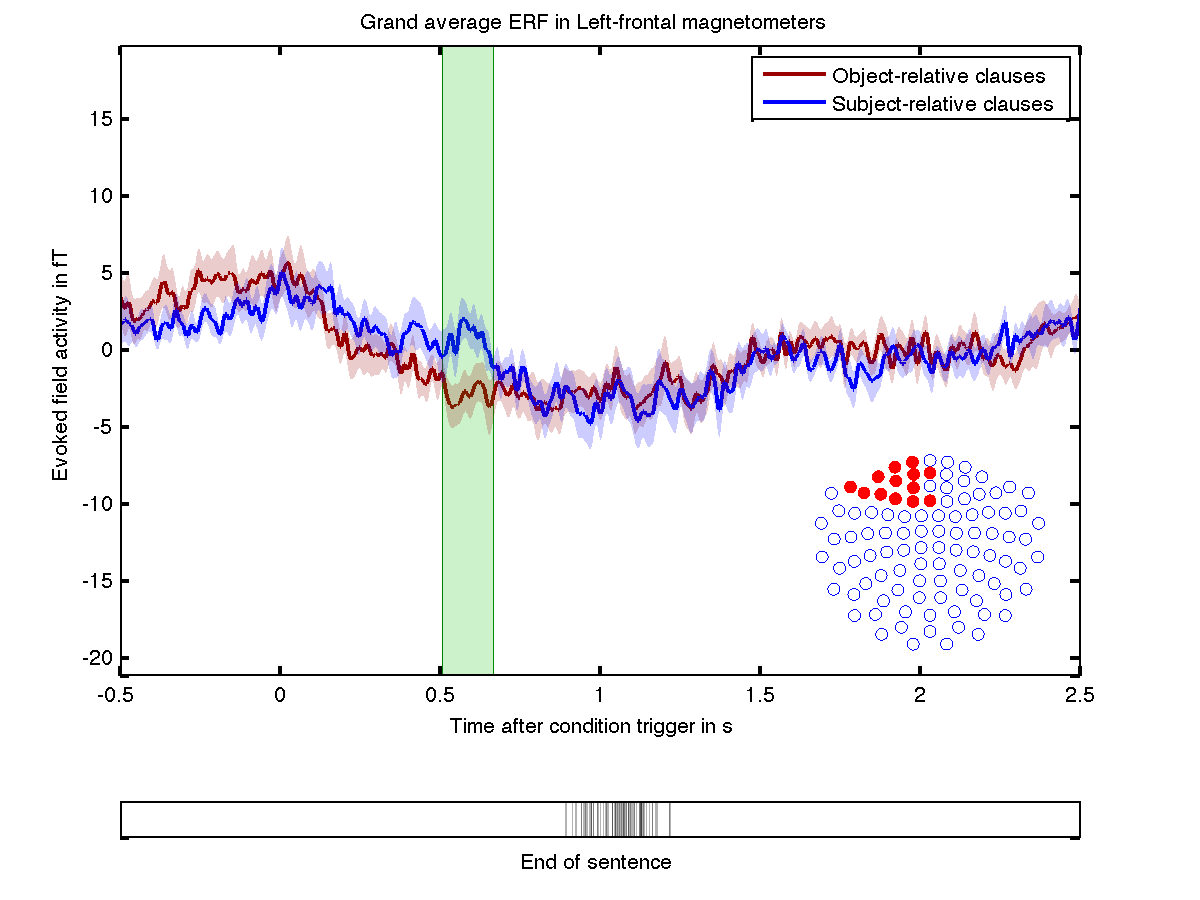
\includegraphics[width=0.49\textwidth]{pics/children_Left-frontal-magnetometers.png}
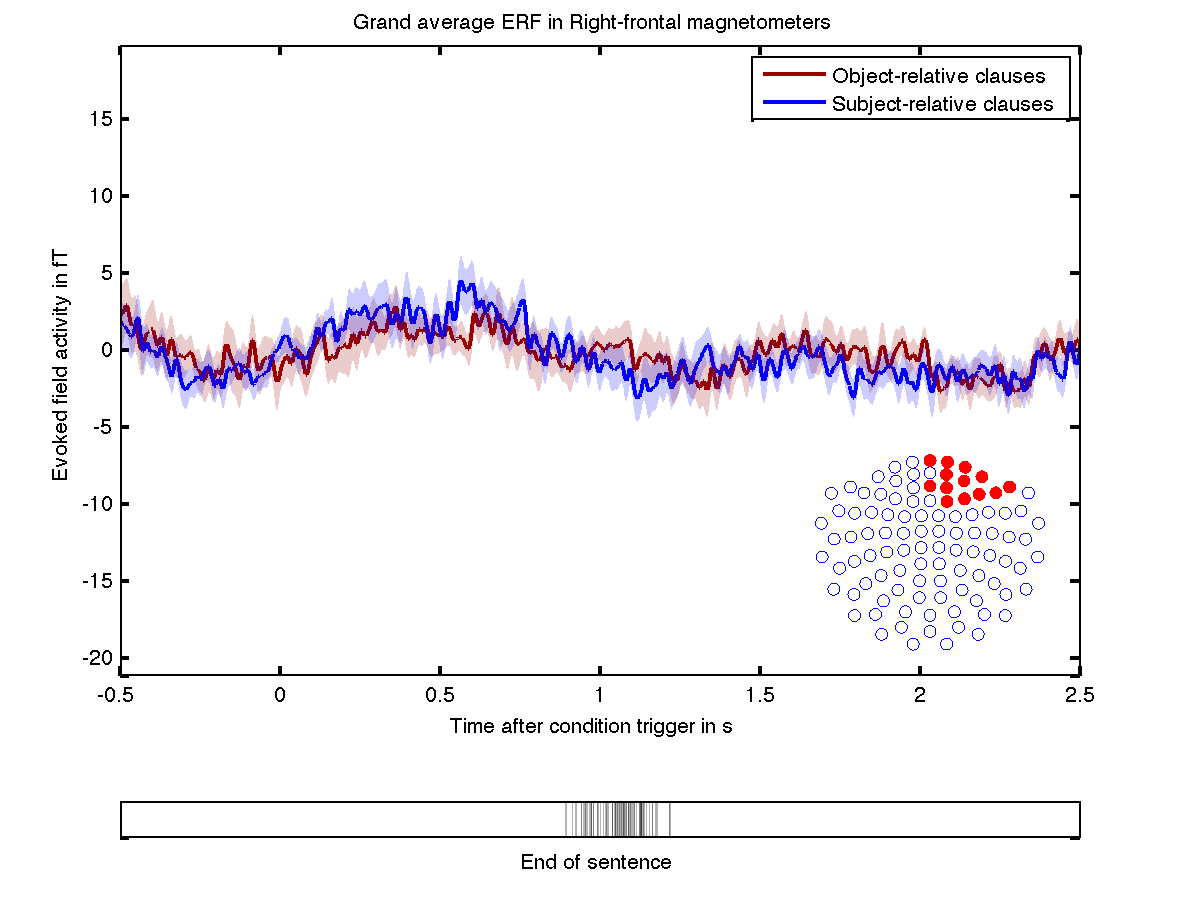
\includegraphics[width=0.49\textwidth]{pics/children_Right-frontal-magnetometers.png}
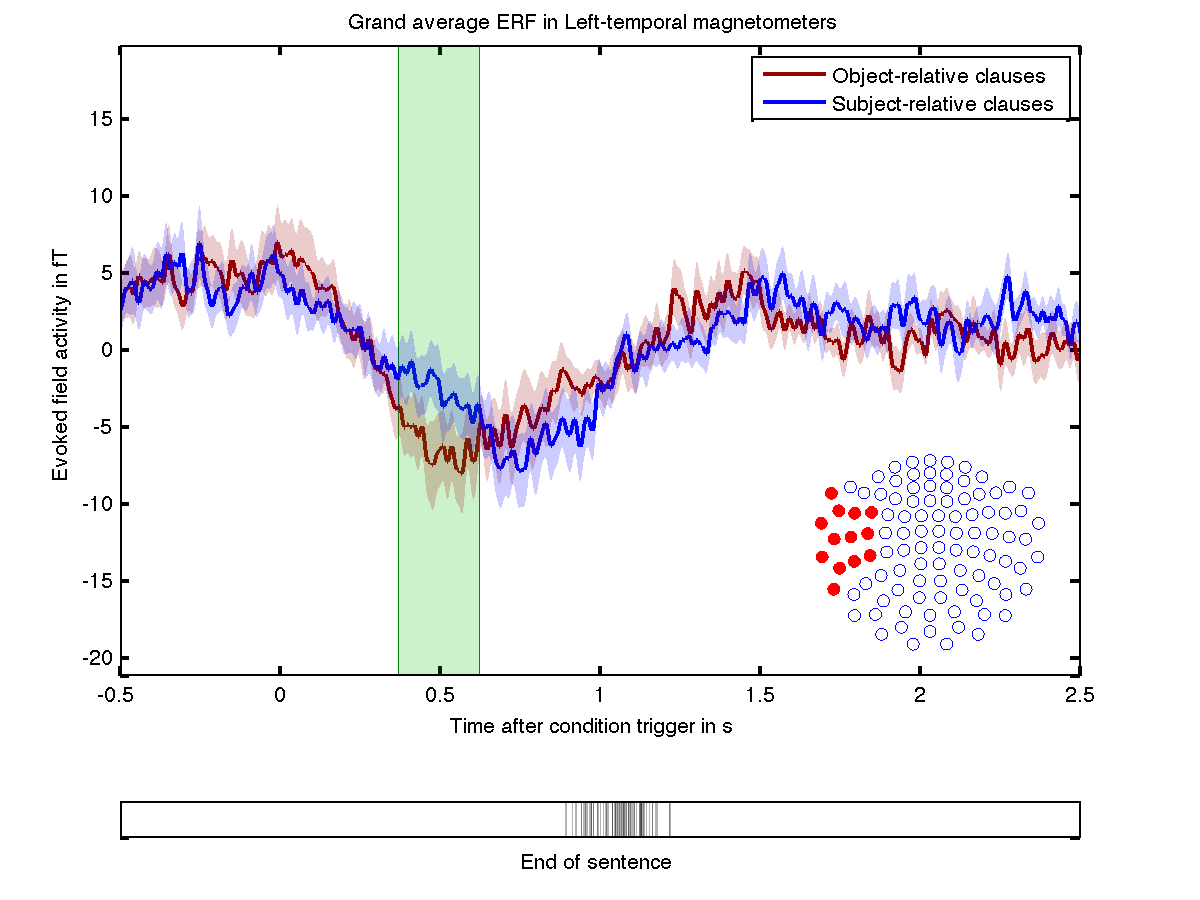
\includegraphics[width=0.49\textwidth]{pics/children_Left-temporal-magnetometers.png}
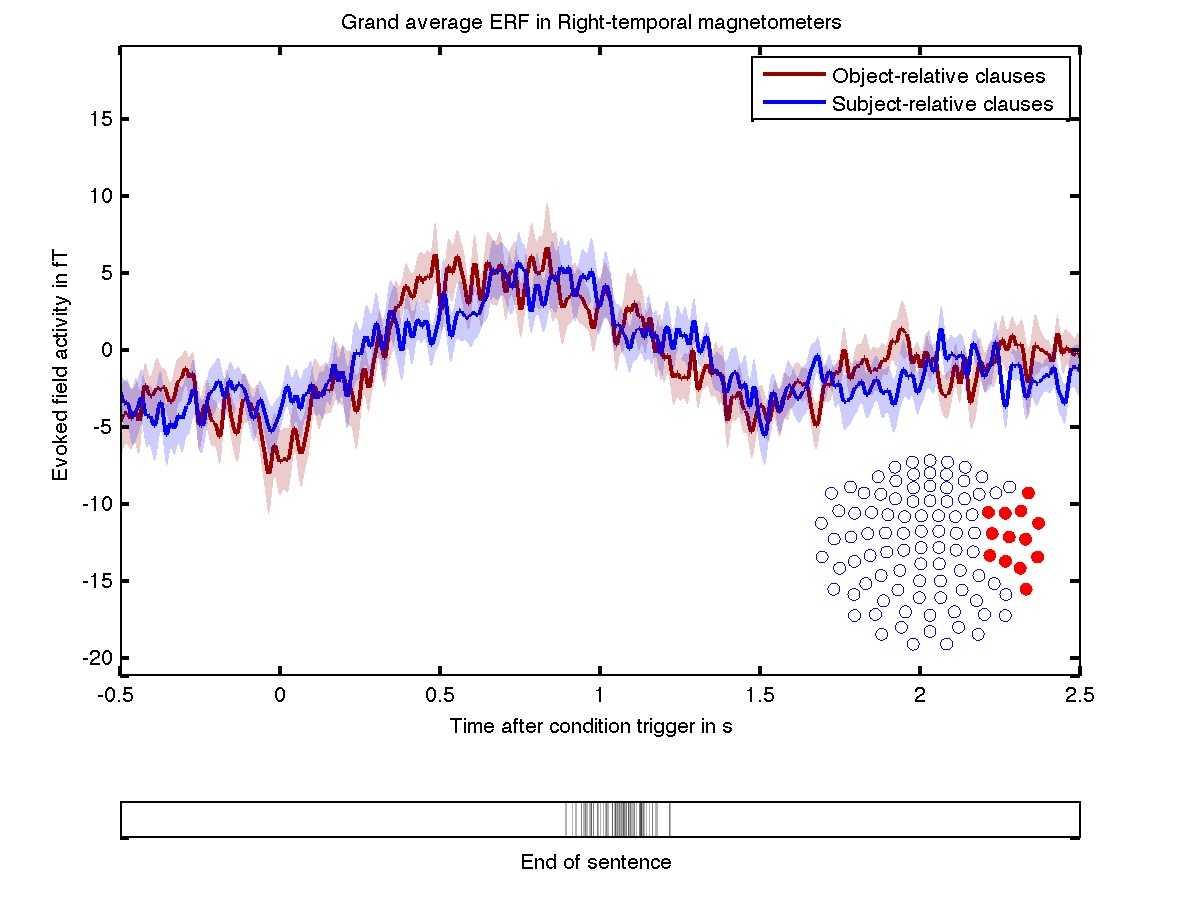
\includegraphics[width=0.49\textwidth]{pics/children_Right-temporal-magnetometers.png}
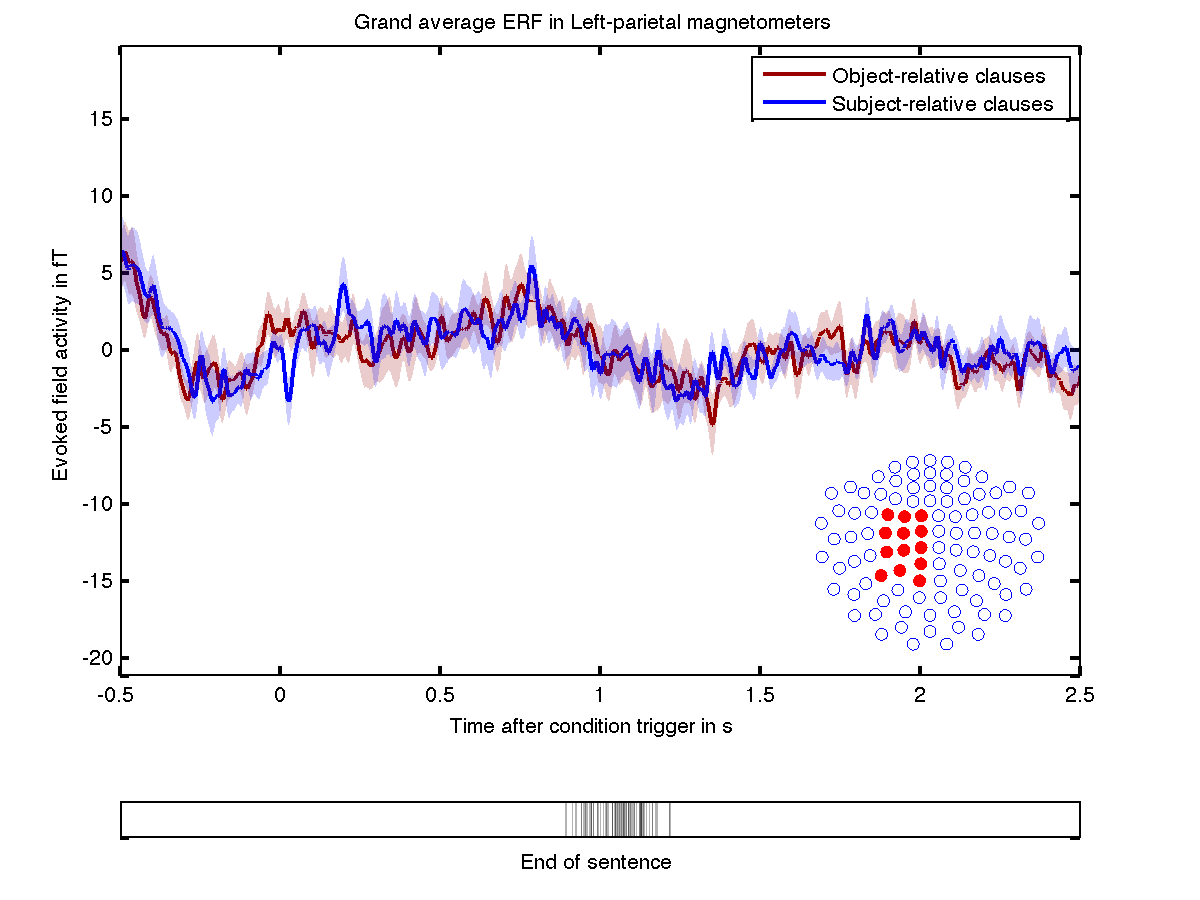
\includegraphics[width=0.49\textwidth]{pics/children_Left-parietal-magnetometers.png}
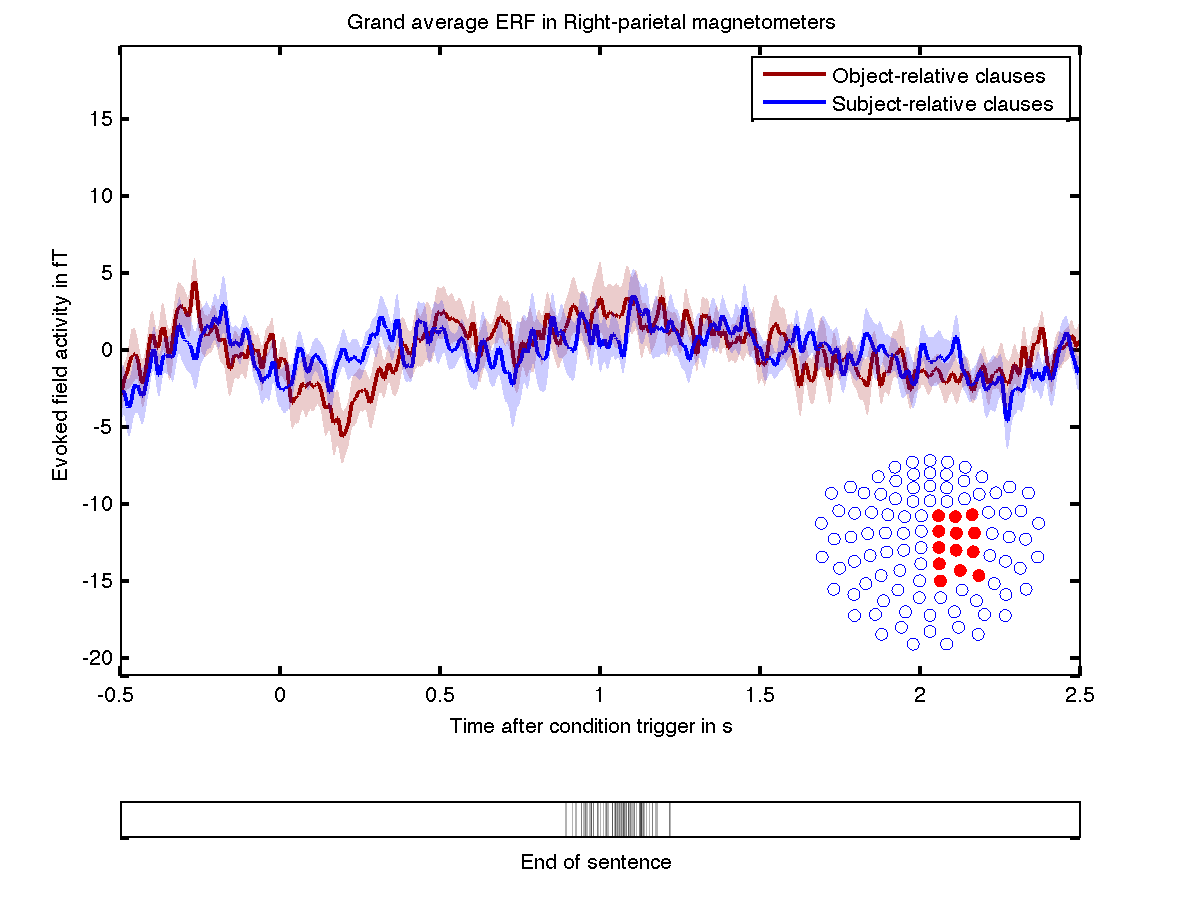
\includegraphics[width=0.49\textwidth]{pics/children_Right-parietal-magnetometers.png}
\caption{\label{4.2.activity.kids} Combined activity from children in separate sensor groups. Only magnetometers are displayed. Top: frontal sensor activity; middle: temporal sensor activity; bottom: parietal sensor activity}
\end{center}
\end{figure}

For adults, clusters of significant differences were observed by left-temporal gradiometers and left-parietal magnetometers.
Left frontal gradiometers showed a weak positive effect between 131ms and 284ms ($p = 6.3\%$).
Left temporal gradiometers showed a positive effect between 257ms and 480ms ($p = 2.1\%$).
Left parietal magnetometers showed a positive effect between 618ms and 765ms ($p = 0.64\%$).
Right temporal magnetometers showed a weak negative effect between 992 and 1154ms ($p = 7.1\%$).
This activity can be roughly categorized into three time windows: two positive effects between 131 and 480ms, 618 and 765ms, and a negative effect between 992 and 1154ms.
The generally lower significance levels imply an overall weaker impact of syntactic condition on sensor activity.

\begin{figure}[h]
\begin{center}
\vspace{7mm}
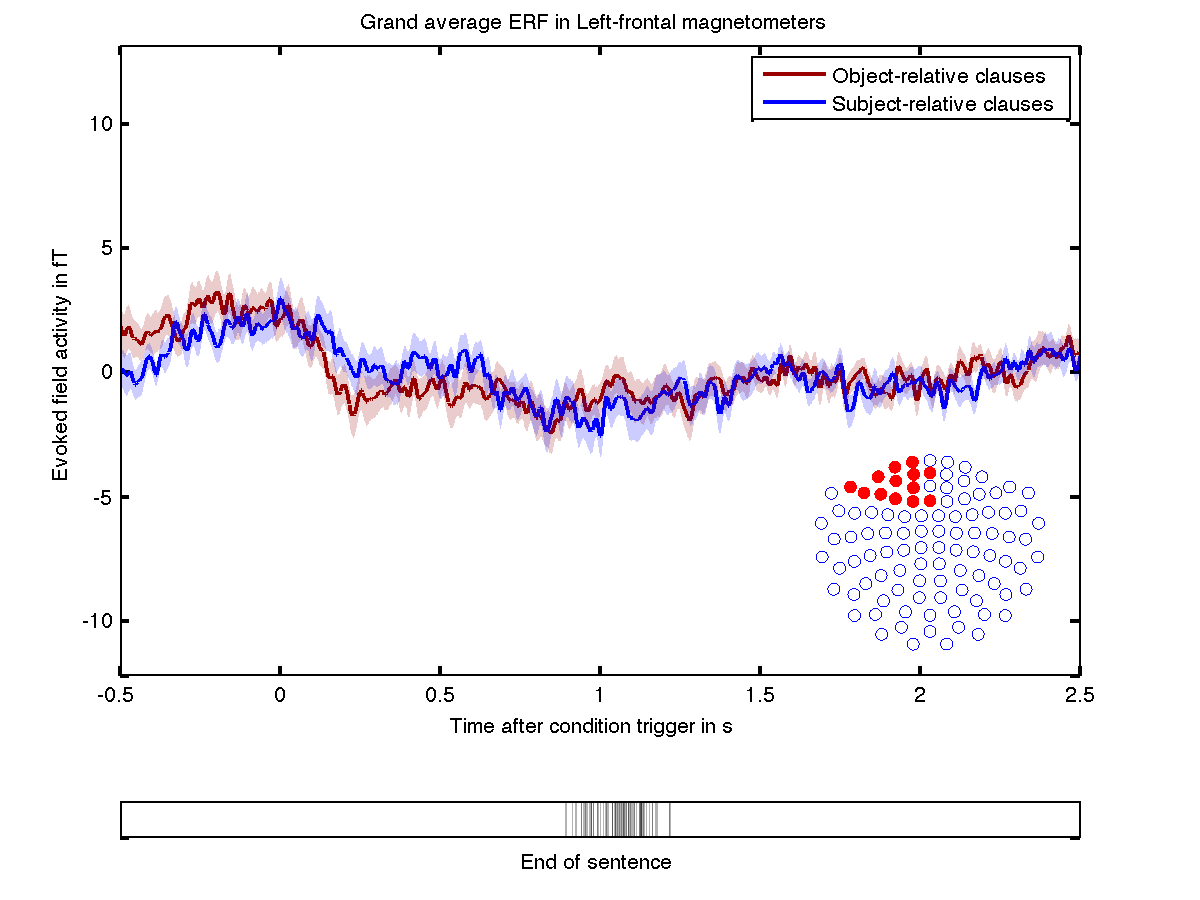
\includegraphics[width=0.49\textwidth]{pics/adults_Left-frontal-magnetometers.png}
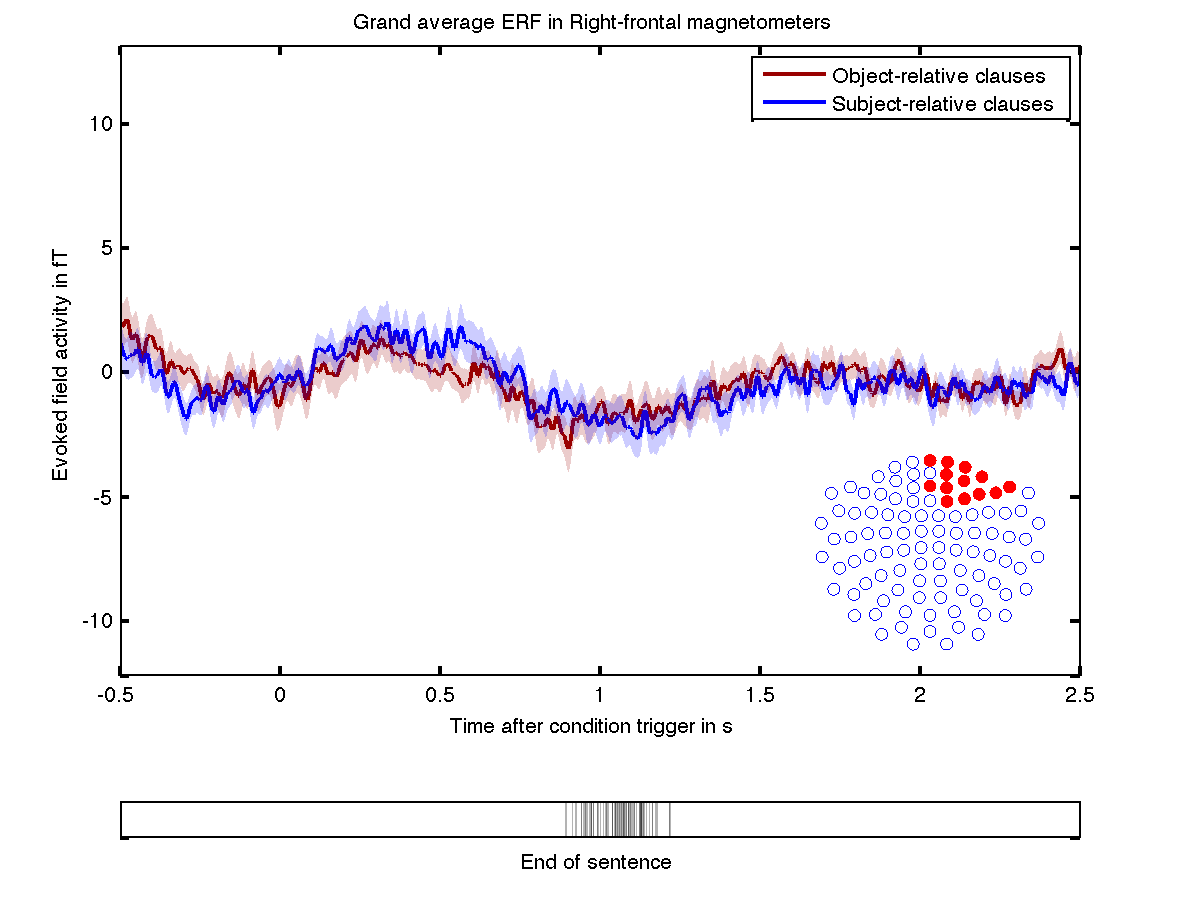
\includegraphics[width=0.49\textwidth]{pics/adults_Right-frontal-magnetometers.png}
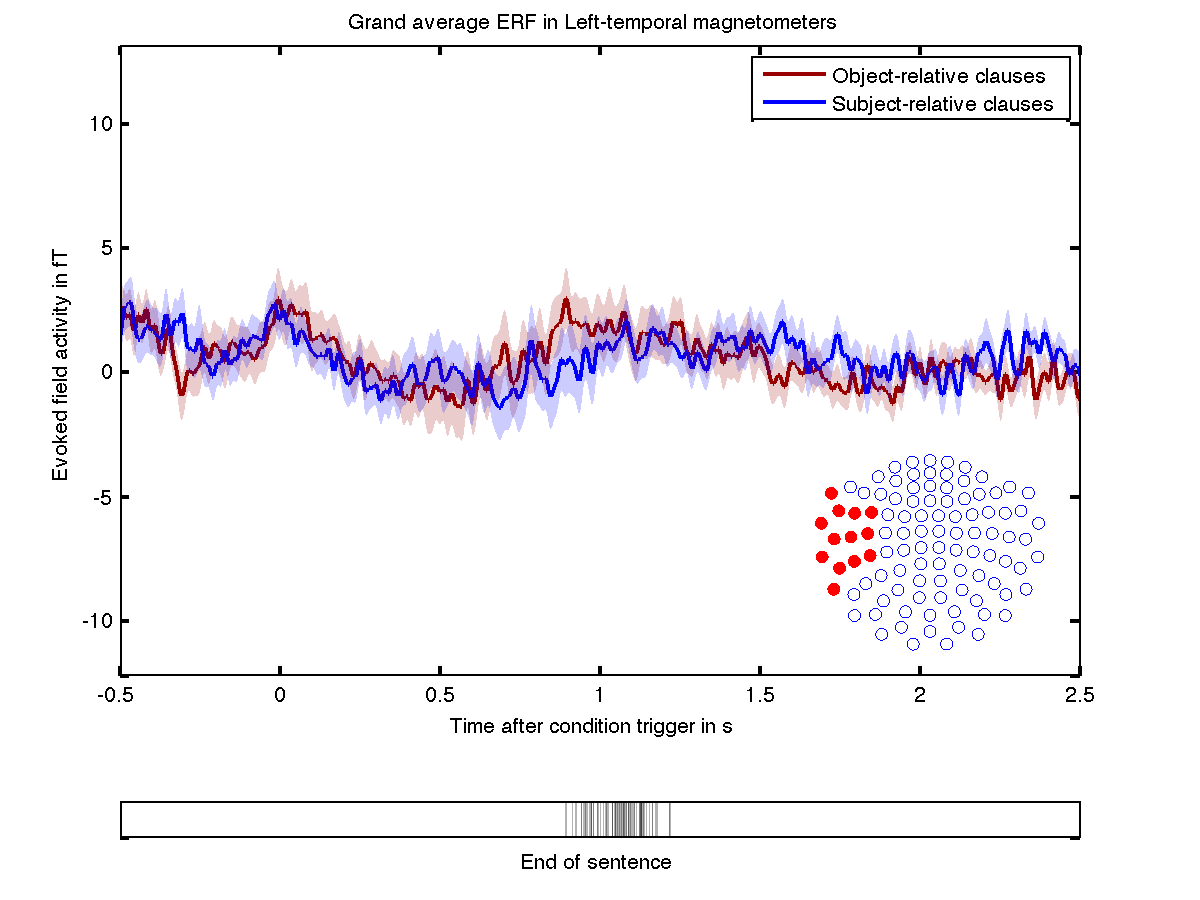
\includegraphics[width=0.49\textwidth]{pics/adults_Left-temporal-magnetometers.png}
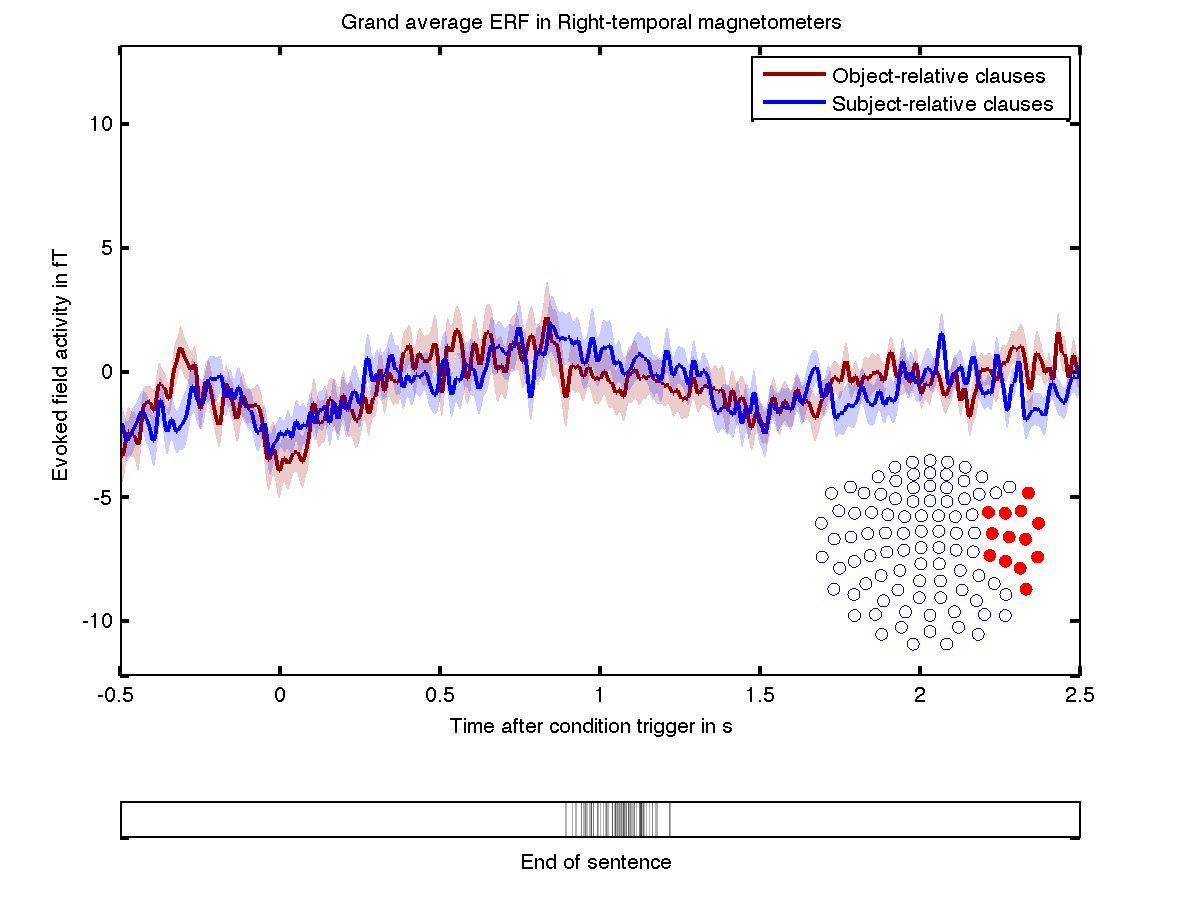
\includegraphics[width=0.49\textwidth]{pics/adults_Right-temporal-magnetometers.png}
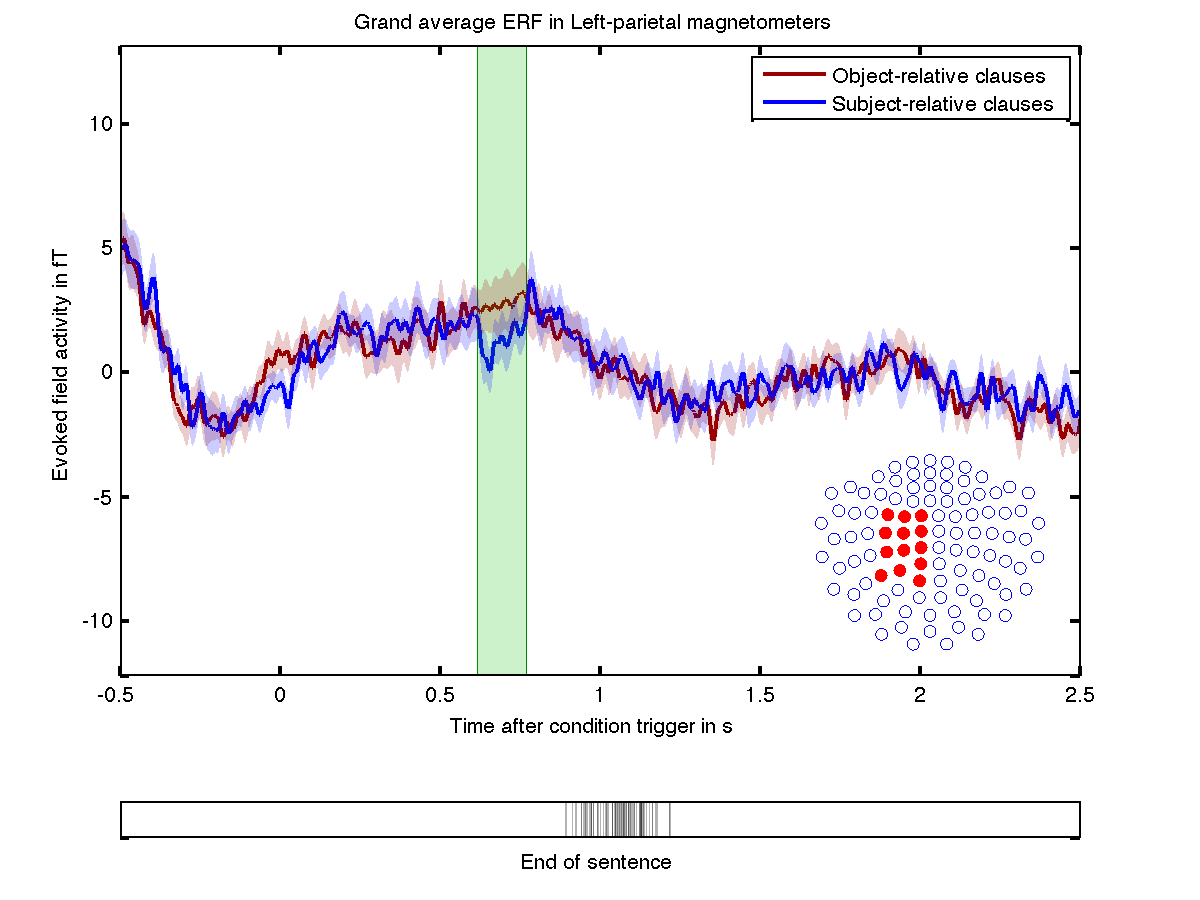
\includegraphics[width=0.49\textwidth]{pics/adults_Left-parietal-magnetometers.png}
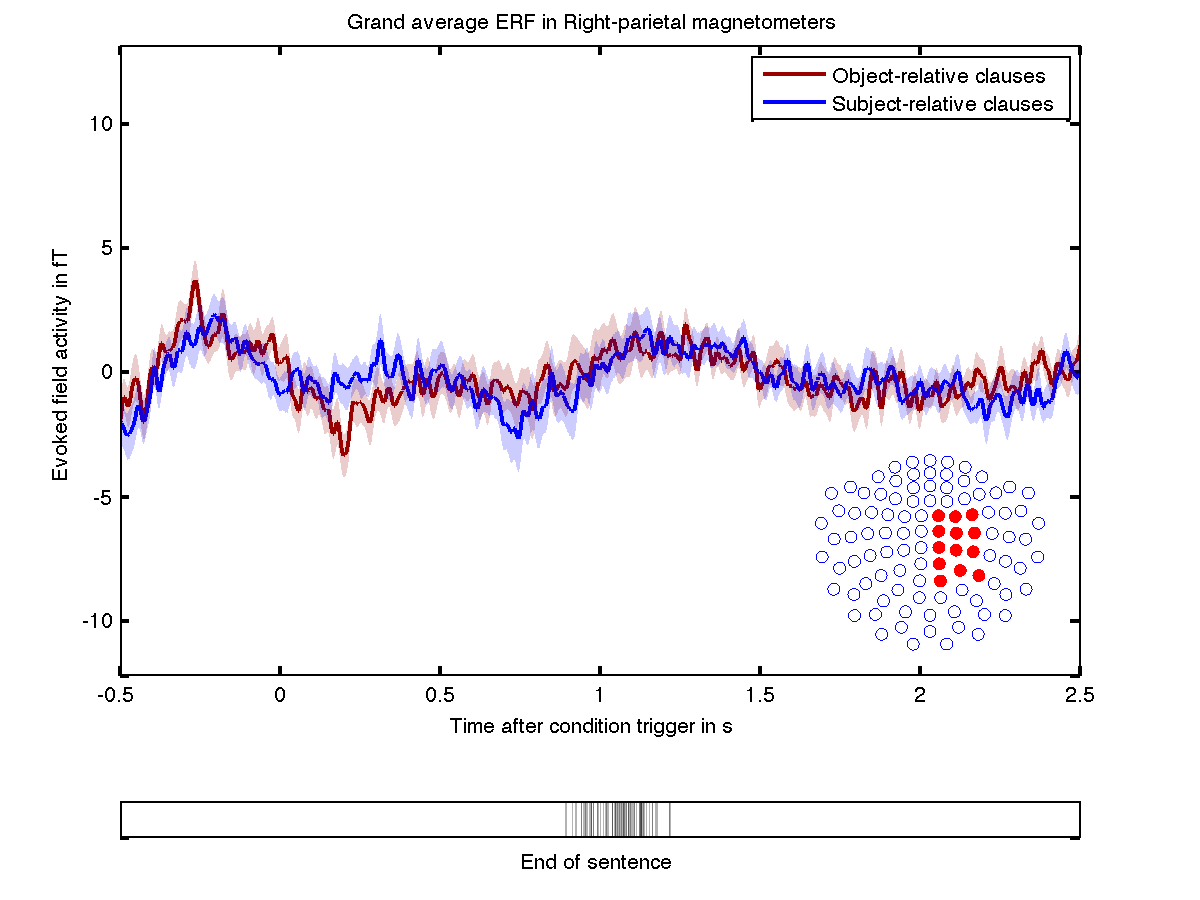
\includegraphics[width=0.49\textwidth]{pics/adults_Right-parietal-magnetometers.png}
\caption{\label{4.2.activity.adults} Combined activity from adults in separate sensor groups. Only magnetometers are displayed. Top: frontal sensor activity; middle: temporal sensor activity; bottom: parietal sensor activity}
\end{center}
\end{figure}